\clearpage
%//==============================--@--==============================//%
\subsection[3.2 Transístor MOS (MOSFET)]{\hspace*{0.075 em}\raisebox{0.2 em}{$\pmb{\drsh}$} Transístor MOS (MOSFET)}
\label{subsec:transistor-MOS}

O \textbf{transístor de efeito de campo} (\textit{Field Effect Transistor}, acrónimo FET) tem esta designação porque o estado de corte ou de condução é determinado pelo campo elétrico no seu interior. A corrente deve-se a um só tipo de portadores de carga (eletrões ou lacunas), ao contrário do que se sucede com os BJT.

Existem vários tipos de transístores de efeito de campo, dos quais o mais utilizado é, de longe, o transístor \textbf{MOS} (MOSFET); a designação MOS provém das iniciais de Metal-Oxide-Semicondutor. 

\vspace{0.5em}
\noindent Algumas considerações pertinentes:
\begin{itemize}[leftmargin=*, nolistsep, itemsep=1pt, label=\rule{0.9ex}{0.9ex}]
    \item Os transístores MOS ocupam menor área, apresentam uma resistência de entrada praticamente infinita, funcionam melhor como interruptores e permitem realizar circuitos digitais com menor consumo (afinidade à realização de circuitos digitais).
    
    \item Os transístores bipolares permitem obter maior ganho, maior largura de banda e precisão mais elevada (especialmente vocacionados para a realização de circuitos analógicos). 

    \item No entanto, \underline{esta separação} dos domínios de aplicação dos dois tipos de transístores está atualmente \underline{ultrapassada}.

    \item Os transístores MOS, inicialmente usados em circuitos lógicos e memórias, são também usados correntemente na realização de circuitos analógicos (descobriram-se formas engenhosas de implementar funções digitais e analógicas quase exclusivamente com MOSFETs $[$i.e., com muito poucas ou nenhumas resistências$]$).

    \item Os transitares bipolares continuam a ser usados na realização de circuitos analógicos e são também usados na realização de circuitos digitais, principalmente se estes tiverem de ser muito rápidos. 

    \item Existem atualmente tecnologias \textbf{BiCMOS}, que combinam, no mesmo circuito integrado, transístores bipolares e CMOS.
\end{itemize}

\begin{figure}[H]
    \begin{subfigure}[b]{0.5\linewidth}
        \centering
        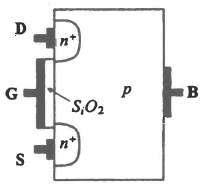
\includegraphics[width = 0.6\linewidth]{img/3/MOSFET/NMOS-enhancement.png}
        \caption{NMOS de reforço}
        \label{fig:NMOS-enhancement}
    \end{subfigure}
    \begin{subfigure}[b]{0.5\linewidth}
        \centering
        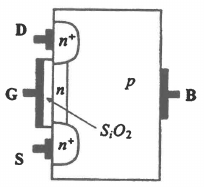
\includegraphics[width = 0.6\linewidth]{img/3/MOSFET/NMOS-depletion.png}
        \caption{NMOS de depleção}
        \label{fig:NMOS-depletion}
    \end{subfigure}%%
    \caption{Estrutura física dos transístores NMOS de reforço e de depleção}
    \label{fig:NMOS}
\end{figure}

\noindent A estrutura básica de um MOSFET inclui um \textbf{substrato} ou corpo (\textit{body}), sobre o qual estão o \textbf{dreno} (\textit{drain}) e a \textbf{fonte} (\textit{source}), áreas altamente concentradas de um tipo de semicondutor. Entre o dreno e a fonte, há uma camada isolante de óxido de silício (SiO$_{2}$), e acima desta, uma camada condutora que constitui a \textbf{porta} (\textit{gate}). 

A corrente flui do dreno para a fonte quando a tensão entre a porta e a fonte, $v_{GS}$, é superior à \textbf{tensão de limiar} (\textit{threshold}), $V_{t}$, formando assim um \textbf{canal}\footnotemark[7] condutor.

\footnotetext[7]{%
    Nos transístores MOS de \textbf{reforço} (\textit{enhancement}) o controlo da corrente obtém-se ao trazer mais ou menos portadores de carga para o canal. Para os MOS de \textbf{depleção}  (\textit{depletion}), o canal é criado durante a fabricação do circuito; o controlo faz-se afastando mais ou menos portadores de carga.
}

\newpage
\noindent \textbf{Notas sobre o funcionamento} dos MOSFET:
\begin{itemize}[leftmargin=*, nolistsep, itemsep=1pt, label=\rule{0.9ex}{0.9ex}]
    \item Contrariamente ao que se verifica nos transístores bipolares, os MOSFET de baixa potência têm uma \underline{estrutura simétrica} (os transístores MOS de potência são assi- métricos). Assim, o dreno e a fonte são determinados pela polaridade da tensão existente entre eles. 

    \item Devido à presença da camada isolante sob a porta, o terminal desta não é percorrido por corrente, i.e., $i_G = 0$. O substrato também não apresenta corrente, porque as suas junções com o dreno e a fonte estão polarizadas em sentido inverso. 
    
    (Normalmente o substrato está ligado à fonte, ou ao terminal negativo da alimentação)

    \item Como $i_G = 0$ e $i_B = 0$, \underline{as correntes na fonte e no dreno são iguais}, $i_D = i_S$.
\end{itemize}

\begin{mdframed}
    \noindent Existem múltiplos \textbf{símbolos} utilizados para representar os transístores MOS. Na \hyperref[fig:MOS-simbolos]{figura seguinte} apresenta-se a simbologia mais antiga (em cima), e a representação frequentemente utilizada atualmente (em baixo).

    \begin{figure}[H]
        \centering
        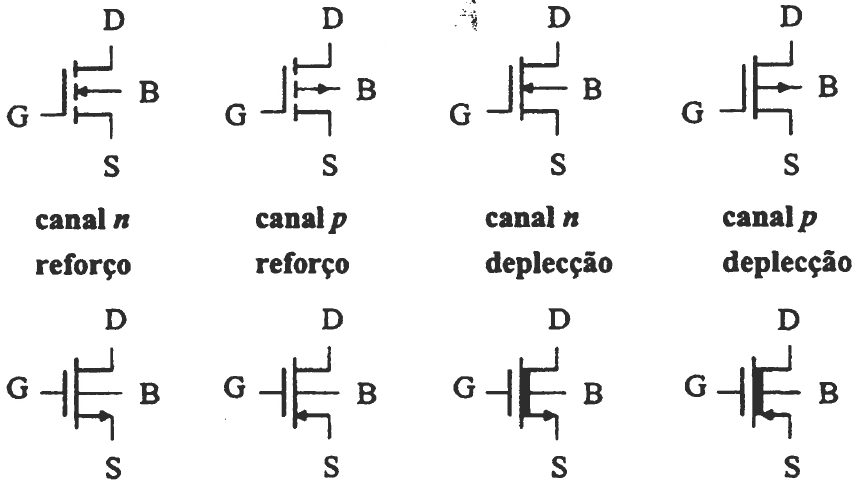
\includegraphics[width=0.7\linewidth]{img/3/MOSFET/MOS-simbolos.png}
        \caption{Símbolos dos transístores MOS \cite{medeiros:CTBM}}
        \label{fig:MOS-simbolos}
    \end{figure}

    \noindent Quando não é necessário indicar o terminal do substrato, recorre-se à representação \textbf{simplificada}, que o omite (dado que não é percorrido por corrente e é ligado à fonte ou a uma tensão fixa):

    \begin{figure}[H]
        \centering
        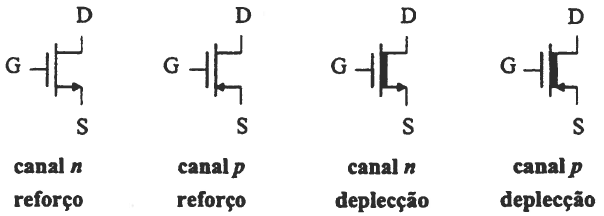
\includegraphics[width=0.65\linewidth]{img/3/MOSFET/MOS-simbolos-simplificado.png}
        \caption{Representação simplificada dos transístores MOS \cite{medeiros:CTBM}}
        \label{fig:MOS-simbolos-simplificado}
    \end{figure}
\end{mdframed}

%//==============================--@--==============================//%
\newpage
\subsubsection[3.2.1 Modos de funcionamento e características i-v]{$\pmb{\rightarrow}$ Modos de funcionamento e características $\mathbf{i-v}$}

\vspace{-0.75em}
\begin{figure}[H]
    \centering
    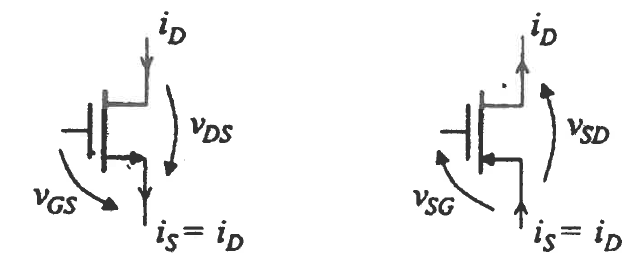
\includegraphics[width=0.55\linewidth]{img/3/MOSFET/MOS-sentidos.png}
    \caption{Sentidos de referência \cite{medeiros:CTBM}. Os sentidos de referência adotados foram escolhidos de forma a que as correntes sejam sempre positivas. Não há corrente aos terminais da porta e do substrato, $i_G = i_B = 0$.}
    \label{fig:MOS-sentidos}
\end{figure}

\vspace{-0.75em}
\noindent Os sentidos de referência para os transístores de depleção são iguais aos apresentados para os transístores de reforço. No entanto, a tensão de limiar $V_t$ passa a ser negativa, podendo os transístores conduzir com $v_{GS} < 0$ ou $v_{SG} < 0$, desde que estas tensões sejam superiores a $V_t$.

\phantomsection\addcontentsline{toc}{paragraph}{Zonas de funcionamento}
\begin{theo}[\underline{Zonas de funcionamento}]{def:MOS-zonas}\label{def:MOS-zonas}
    \begin{itemize}[leftmargin=*]
        \item[] \textbf{(i) Corte:} \hfill $\boxed{ v_{GS} < V_t \rightarrow i_D = i_S = 0}$ \\[1pt]
        Não existem\footnotemark[8] portadores entre D e S
        
        \item[] \textbf{(ii) Condução:} \hfill $\boxed{ v_{GS} > V_t \rightarrow i_D = i_S \neq 0}$ \\[1pt]
        Quando os transístores MOS conduzem podem situar-se em duas regiões de funcionamento: \\
        Região de \textbf{tríodo} (ou óhmica) e a região de \textbf{saturação} (ou de estrangulamento).
        
        \begin{itemize}[label=\rule{0.9ex}{0.9ex}]
            \item O transístor NMOS está na região de \textbf{tríodo} \hfill $\boxed{ v_{DS} < v_{GS} - V_t }$

            Neste caso a corrente é dada por
            $$
                \boxed{ i_D = k\left[ 2(v_{GS} - V_t)v_{DS} - v_{DS}^2 \right] }
            $$
            em que $k$ é um parâmetro dependente do material e da geometria do transístor.

            Note-se que para tensões $v_{DS} \ll v_{GS} - V_t$, o transístor comporta-se como uma resistência $R_{DS}$ comandada pela tensão $v_{GS}$:
            $$
                i_D \approx 2k(v_{GS} - V_t)v_{DS} \implies R^{-1}_{DS} = 2k(v_{GS} - V_t)
            $$

            \item O transístor NMOS está na região de \textbf{saturação} \hfill $\boxed{ v_{DS} \ge v_{GS} - V_t }$

            A corrente passa a ser aproximadamente independente de $v_{DS}$:
            $$
                \boxed{ i_D = k\left( v_{GS} - V_t \right)^2 }
            $$
        \end{itemize}
        
    \end{itemize}
\end{theo}
      
\noindent O parâmetro $k$ que figura nas equações anteriores exprime-se em AV$^{-2}$
$$
    \boxed{ k = \frac{1}{2}\, \mu C_{ox} \frac{W}{L} } \;\: \text{em que }\, C_{ox} = \frac{\varepsilon_{ox}}{t_{ox}}\; \text{\footnotesize (capacidade formada entre a porta e o substrato)}
$$

\footnotetext[8]{%
    ``This is not entirely true, for it has been found that for values of $v_{GS}$ smaller than but close to $V_t$, a small drain current flows. In this \textbf{subthreshold} region of operation, the drain current is exponentially related to $v_{GS}$, much like the $i_C-v_{BE}$ relationship of a BJT''\cite{sedra-smith:microelectronic-circuits}
}

\renewcommand*{\thefootnote}{\fnsymbol{footnote}}
\footnotetext[4]{%
    $W$ é a largura (\textit{width}) do transístor, e $L$ o comprimento (\textit{length}). $W/L$ refere-se como \textit{aspect-ratio}.
}
\renewcommand*{\thefootnote}{\arabic{footnote}}
%//==============================--@--==============================//%
\paragraph[3.2.1.1 Características i-v]{$\pmb{\star}$ Características $\mathbf{i-v}$}\mbox{}\\[4pt]
A representação gráfica das características $i_D(v_{DS})$ para diferentes valores de $v_{GS}$ é acompanhada pela região de fronteira entre as regiões tríodo e de saturação

\vspace{-0.75em}
$$
    v_{DS} = v_{GS} - V_t\;\; \text{donde resulta}\;\; i_D = k\, v^2_{DS}
$$

\vspace{-0.75em}
\begin{figure}[H]
    \begin{subfigure}[b]{0.5\linewidth}
        \centering
        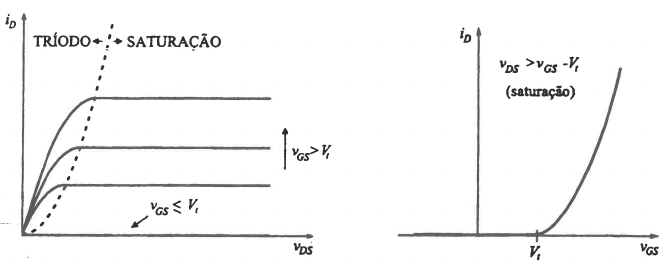
\includegraphics[width = 0.95\linewidth]{img/3/MOSFET/i-v-enhancement.png}
        \caption{Características do NMOS de reforço}
        \label{fig:NMOS-i-v-enhancement}
    \end{subfigure}
    \begin{subfigure}[b]{0.5\linewidth}
        \centering
        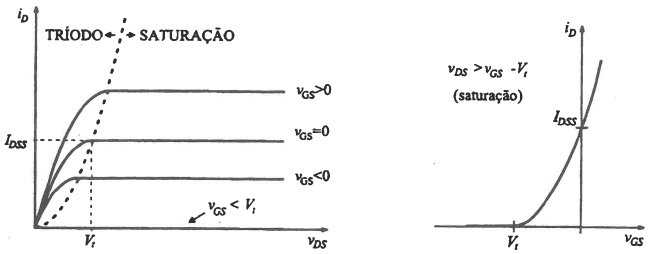
\includegraphics[width = 0.95\linewidth]{img/3/MOSFET/i-v-depletion.png}
        \caption{Características do NMOS de depleção}
        \label{fig:NMOS-i-v-depletion}
    \end{subfigure}%%
    \caption{Características $i-v$ para o transístor NMOS}
    \label{fig:NMOS-i-v}
\end{figure}

\noindent Os transístores de depleção têm as mesmas equações que os de reforço, mas como mencionado anteriormente, a tensão de limiar $V_t$ é negativa. Desta forma, costuma representar-se $I_{DSS} = kV^2_t$ (\textit{drain current for zero bias}), o valor de $i_D$ quando $v_{GS} = 0$. Para valores de $v_{GS} < 0$, encontra-se no modo de depleção, e para $v_{GS} > 0$ no de reforço. 

\begin{figure}[H]
    \centering
    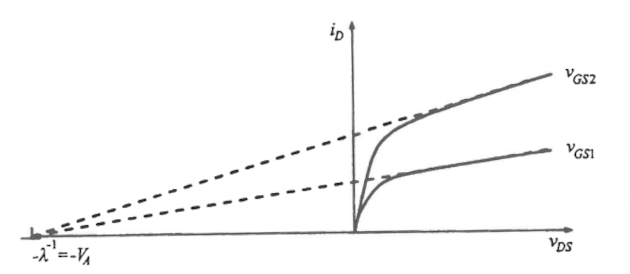
\includegraphics[width = 0.6\linewidth]{img/3/MOSFET/MOS-early-effect.png}
    \caption{Efeito de $v_{DS}$ sobre $i_{D}$ na saturação \cite{medeiros:CTBM}}
    \label{fig:MOS-early-effect}
\end{figure}

\noindent Na realidade, a tensão $v_{DS}$ tem alguma influência em $i_D$. Isto resulta do fenómeno designado por \underline{modulação do comprimento do canal}, cujas consequências são semelhantes ao efeito de Early (modulação da espessura da base) nos BJT.

Caso se considere este efeito, a característica \underline{na região de saturação} passa a ser
$$
    \boxed{ i_D = k\left( v_{GS} - V_t \right)^2 (1 + \lambda v_{DS}) }
$$
em que o parâmetro $\lambda^{-1} = V_A$ é equivalente à tensão de Early nos transístores bipolares.

%//==============================--@--==============================//%
\paragraph[3.2.1.2 Efeito da Temperatura]{$\pmb{\star}$ Efeito da Temperatura}\mbox{}\\[4pt]
Os parâmetros $V_t$ e $k$ que caracterizam o transístor MOS são sensíveis à temperatura: a tensão de limiar $V_t$, diminui cerca de $2$mV/\textdegree{C}; o parâmetro $k$ também diminui com a temperatura, e o seu efeito sobre $i_D$ opõe-se e predomina sobre o da variação de $V_t$. Assim, com $i_D$ constante, $v_{GS}$ aumenta com a temperatura. Note-se que este efeito é ao contrário do que acontece no transístor bipolar, em que, com $i_C$ constante, $v_{BE}$ diminui quando aumenta a temperatura.

%//==============================--@--==============================//%
\newpage
\paragraph[3.2.1.3 Efeito de Corpo]{$\pmb{\star}$ Efeito de Corpo (\textit{Body Effect})}\mbox{}\\[4pt]
O \textbf{efeito de corpo}, ou \textit{body effect}, relaciona a alteração da tensão de limiar do dispositivo, $V_t$, com a tensão aplicada ao substrato (ou corpo). Esta alteração é especialmente notável quando o substrato não está ligado ao \textit{ground} ou está ligado a um potencial diferente do terminal da fonte.

\begin{mdframed}
    \noindent A tensão de limiar modificada devido ao \textbf{efeito de corpo} é representada por:
    
    $$
        \boxed{ V_t = V_{t0} + \gamma \left[ \sqrt{{2\phi_f + v_{SB}}} - \sqrt{{2\phi_f}} \right] }
    $$
    
    \noindent em que:
    \begin{itemize}[noitemsep, nolistsep]
        \item $V_{t0}$ é a tensão de limiar \underline{sem o efeito de corpo}.
        \item $\gamma$ é o coeficiente do efeito de corpo, também conhecido como parâmetro de modulação do substrato (depende da técnologia).
        \item $\phi_f$ é o potencial de Fermi.
    \end{itemize}
    
    \vspace{0.5em}
    \noindent A equação acima indica que a tensão de limiar aumenta com o aumento de $v_{SB}$. Este efeito é normalmente indesejável em aplicações analógicas, porque introduz não-linearidades. Em aplicações digitais, onde os transístores operam em modo de corte ou saturação, o efeito é menos relevante.
\end{mdframed}

%//==============================--@--==============================//%
\subsubsection[3.2.2 Modelo incremental]{$\pmb{\rightarrow}$ Modelo incremental}

À semelhança da discussão realizada para os BJT, se o transístor permanecer na região de saturação temos
$$
    \begin{aligned}
        i_D = (I_D + i_d) &= k(V_{GS} + v_{gs} - V_t)^2\\
        &= k(V_{GS} - V_t)^2 + 2k(V_{GS} - V_t) v_{gs} + k v^2_{gs}
    \end{aligned}
$$
\noindent como $I_D = k(V_{GS} - V_t)^2$, fica
$$
    i_d = 2k (V_{GS} - V_t)v_{gs} + k v^2_{gs}
$$
O funcionamento é linear do ponto de vista incremental se $v_{gs} \ll V_{GS} - V_t$, obtendo-se
$$
    i_d = g_m v_{gs}
$$
em que a \textbf{transcondutância} $g_m$, é dada por
$$
    g_m = 2k(V_{GS} - V_t) \iff g_m = 2\sqrt{k I_D}
$$
Se considerarmos o efeito de $v_{DS}$ sobre $i_D$, a transcondutância define-se como
$$
    g_m = \left.\frac{\partial i_D}{\partial v_{GS}}\right|_{v_{GS} = V_{GS};\; v_{DS} = V_{DS}} = 2k(V_{GS} - V_t)(1 + \lambda V_{DS}) = \frac{2 I_D}{V_{GS} - V_t}
$$
\noindent \textbf{Nota:} se $\lambda V_{DS} \ll 1$, o resultado coincide com o anterior, como seria esperado.

\vspace{0.5em}
\noindent Para se ter em conta o efeito de $v_{ds}$ sobre $i_d$ é necessário introduzir o parâmetro incremental
$$
    r^{-1}_o = \left.\frac{\partial i_D}{\partial v_{DS}}\right|_{v_{GS} = V_{GS};\; v_{DS} = V_{DS}} \implies r_o = \frac{1 + \lambda V_{DS}}{\lambda I_D} \;\overset{\scriptstyle \lambda V_{DS} \ll 1}{\simeq}\; \frac{1}{\lambda I_D} = \frac{V_A}{I_D}
$$

\newpage
\noindent Se o \textbf{efeito de corpo} não for desprezável, i.e., a tensão entre a fonte e o substrato não for constante, $v_{bs} \neq 0$, representa-se no esquema incremental um gerador de corrente comandado extra, com parâmetro incremental $g_{mb}$ que se situa entre $0.1 g_m$ e $0.3 g_m$:
$$
    g_{mb} = \left.\frac{\partial i_D}{\partial v_{BS}}\right|_{v_{GS} = V_{GS};\; v_{DS} = V_{DS};\; v_{BS} = V_{BS}}
$$

\begin{figure}[H]
    \begin{subfigure}[b]{0.5\linewidth}
        \centering
        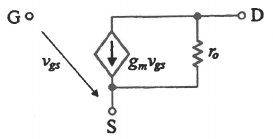
\includegraphics[width = 0.85\linewidth]{img/3/MOSFET/MOS-esquema-ro.png}
        \caption{Com o efeito de $v_{ds}$ sobre $i_d$ ($\lambda \neq 0$)}
        \label{fig:MOS-esquema-ro}
    \end{subfigure}
    \begin{subfigure}[b]{0.5\linewidth}
        \centering
        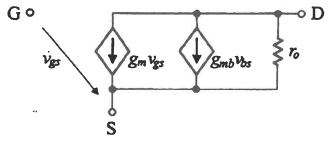
\includegraphics[width = \linewidth]{img/3/MOSFET/MOS-esquema-body.png}
        \caption{Quando há efeito de corpo}
        \label{fig:MOS-esquema-body-effect}
    \end{subfigure}%%
    \caption{Esquemas incrementais para os transístores MOS \cite{medeiros:CTBM}}
    \label{fig:MOS-esquema-incremental}
\end{figure}

\begin{mdframed}
    \begin{quote} \small
        ``É oportuno fazer a comparação das transcondutâncias dos transístores bipolar e MOS. $[$Sem o efeito de corpo temos:$]$
        $$
            \frac{(g_m)_{BJT}}{(g_m)_\text{MOS}} = \frac{I_C/V_T}{2 I_D/(V_{GS} - V_t)}
        $$
        e se $I_C = I_D$, fica
        $$
            \frac{(g_m)_{BJT}}{(g_m)_\text{MOS}} = \frac{V_{GS} - V_t}{2 V_T}
        $$
        Como $2V_T \approx 50$mV e $(V_{GS} - V_t)$ é da ordem de grandeza de $1$V, conclui-se que, para o mesmo nível de corrente em repouso, o transístor bipolar tem uma transcondutância que é algumas dezenas de vezes superior à do transístor MOS. Por exemplo, se $V_{GS} - V_t = 2$V, obtém-se $(g_m)_\text{BJT} = 40(g_m)_\text{MOS}$. A esta significativa desvantagem do transístor MOS, contrapõem-se os aspetos em que é superior: resistência de entrada infinita, menor área de circuito integrado, processo de fabricação mais simples.''\cite{medeiros:CTBM}
    \end{quote}
\end{mdframed}
%//==============================--@--==============================//%